\documentclass[twoside]{book}

% Packages required by doxygen
\usepackage{fixltx2e}
\usepackage{calc}
\usepackage{doxygen}
\usepackage[export]{adjustbox} % also loads graphicx
\usepackage{graphicx}
\usepackage[utf8]{inputenc}
\usepackage{makeidx}
\usepackage{multicol}
\usepackage{multirow}
\PassOptionsToPackage{warn}{textcomp}
\usepackage{textcomp}
\usepackage[nointegrals]{wasysym}
\usepackage[table]{xcolor}

% Font selection
\usepackage[T1]{fontenc}
\usepackage[scaled=.90]{helvet}
\usepackage{courier}
\usepackage{amssymb}
\usepackage{sectsty}
\renewcommand{\familydefault}{\sfdefault}
\allsectionsfont{%
  \fontseries{bc}\selectfont%
  \color{darkgray}%
}
\renewcommand{\DoxyLabelFont}{%
  \fontseries{bc}\selectfont%
  \color{darkgray}%
}
\newcommand{\+}{\discretionary{\mbox{\scriptsize$\hookleftarrow$}}{}{}}

% Page & text layout
\usepackage{geometry}
\geometry{%
  a4paper,%
  top=2.5cm,%
  bottom=2.5cm,%
  left=2.5cm,%
  right=2.5cm%
}
\tolerance=750
\hfuzz=15pt
\hbadness=750
\setlength{\emergencystretch}{15pt}
\setlength{\parindent}{0cm}
\setlength{\parskip}{3ex plus 2ex minus 2ex}
\makeatletter
\renewcommand{\paragraph}{%
  \@startsection{paragraph}{4}{0ex}{-1.0ex}{1.0ex}{%
    \normalfont\normalsize\bfseries\SS@parafont%
  }%
}
\renewcommand{\subparagraph}{%
  \@startsection{subparagraph}{5}{0ex}{-1.0ex}{1.0ex}{%
    \normalfont\normalsize\bfseries\SS@subparafont%
  }%
}
\makeatother

% Headers & footers
\usepackage{fancyhdr}
\pagestyle{fancyplain}
\fancyhead[LE]{\fancyplain{}{\bfseries\thepage}}
\fancyhead[CE]{\fancyplain{}{}}
\fancyhead[RE]{\fancyplain{}{\bfseries\leftmark}}
\fancyhead[LO]{\fancyplain{}{\bfseries\rightmark}}
\fancyhead[CO]{\fancyplain{}{}}
\fancyhead[RO]{\fancyplain{}{\bfseries\thepage}}
\fancyfoot[LE]{\fancyplain{}{}}
\fancyfoot[CE]{\fancyplain{}{}}
\fancyfoot[RE]{\fancyplain{}{\bfseries\scriptsize Generated by Doxygen }}
\fancyfoot[LO]{\fancyplain{}{\bfseries\scriptsize Generated by Doxygen }}
\fancyfoot[CO]{\fancyplain{}{}}
\fancyfoot[RO]{\fancyplain{}{}}
\renewcommand{\footrulewidth}{0.4pt}
\renewcommand{\chaptermark}[1]{%
  \markboth{#1}{}%
}
\renewcommand{\sectionmark}[1]{%
  \markright{\thesection\ #1}%
}

% Indices & bibliography
\usepackage{natbib}
\usepackage[titles]{tocloft}
\setcounter{tocdepth}{3}
\setcounter{secnumdepth}{5}
\makeindex

% Hyperlinks (required, but should be loaded last)
\usepackage{ifpdf}
\ifpdf
  \usepackage[pdftex,pagebackref=true]{hyperref}
\else
  \usepackage[ps2pdf,pagebackref=true]{hyperref}
\fi
\hypersetup{%
  colorlinks=true,%
  linkcolor=blue,%
  citecolor=blue,%
  unicode%
}

% Custom commands
\newcommand{\clearemptydoublepage}{%
  \newpage{\pagestyle{empty}\cleardoublepage}%
}

\usepackage{caption}
\captionsetup{labelsep=space,justification=centering,font={bf},singlelinecheck=off,skip=4pt,position=top}

%===== C O N T E N T S =====

\begin{document}

% Titlepage & ToC
\hypersetup{pageanchor=false,
             bookmarksnumbered=true,
             pdfencoding=unicode
            }
\pagenumbering{roman}
\begin{titlepage}
\vspace*{7cm}
\begin{center}%
{\Large Lin\+QT \\[1ex]\large 1.\+0 }\\
\vspace*{1cm}
{\large Generated by Doxygen 1.8.11}\\
\end{center}
\end{titlepage}
\clearemptydoublepage
\tableofcontents
\clearemptydoublepage
\pagenumbering{arabic}
\hypersetup{pageanchor=true}

%--- Begin generated contents ---
\chapter{Bug List}
\label{bug}
\hypertarget{bug}{}

\begin{DoxyRefList}
\item[\label{bug__bug000001}%
\hypertarget{bug__bug000001}{}%
File \hyperlink{compute-DOS_09FFT_8cpp}{compute-\/\+D\+O\+S+\+F\+FT.cpp} ]No know bugs.  
\item[\label{bug__bug000002}%
\hypertarget{bug__bug000002}{}%
File \hyperlink{types__definitions_8hpp}{types\+\_\+definitions.hpp} ]No know bugs. 
\end{DoxyRefList}
\chapter{Module Index}
\section{Modules}
Here is a list of all modules\+:\begin{DoxyCompactList}
\item \contentsline{section}{Kpm}{\pageref{group__kpm}}{}
\end{DoxyCompactList}

\chapter{Namespace Index}
\section{Namespace List}
Here is a list of all documented namespaces with brief descriptions\+:\begin{DoxyCompactList}
\item\contentsline{section}{\hyperlink{namespacekpm}{kpm} }{\pageref{namespacekpm}}{}
\end{DoxyCompactList}

\chapter{File Index}
\section{File List}
Here is a list of all documented files with brief descriptions\+:\begin{DoxyCompactList}
\item\contentsline{section}{/data/jgarcia/lin\+Q\+T/include/\hyperlink{types__definitions_8hpp}{types\+\_\+definitions.\+hpp} \\*The definitions for the project data types are given in this header }{\pageref{types__definitions_8hpp}}{}
\item\contentsline{section}{/data/jgarcia/lin\+Q\+T/src/\hyperlink{compute-DOS_09FFT_8cpp}{compute-\/\+D\+O\+S+\+F\+F\+T.\+cpp} \\*This defines the compute-\/\+D\+O\+S+\+F\+FT function, which uses the kernel polynomial method and fast-\/fourier transform for computing the density of states in sparse systems }{\pageref{compute-DOS_09FFT_8cpp}}{}
\end{DoxyCompactList}

\chapter{Module Documentation}
\hypertarget{group__kpm}{\section{Kpm}
\label{group__kpm}\index{Kpm@{Kpm}}
}
\subsection*{Namespaces}
\begin{DoxyCompactItemize}
\item 
 \hyperlink{namespaceNumCal_1_1kpm}{Num\+Cal\+::kpm}
\end{DoxyCompactItemize}
\subsection*{Classes}
\begin{DoxyCompactItemize}
\item 
class \hyperlink{classNumCal_1_1ChebyshevSet}{Num\+Cal\+::\+Chebyshev\+Set}
\item 
class \hyperlink{classNumCal_1_1Kpm}{Num\+Cal\+::\+Kpm}
\begin{DoxyCompactList}\small\item\em Set of approximation based on K\+P\+M. \end{DoxyCompactList}\end{DoxyCompactItemize}


\subsection{Detailed Description}

\chapter{Namespace Documentation}
\hypertarget{namespacekpm}{}\section{kpm Namespace Reference}
\label{namespacekpm}\index{kpm@{kpm}}
\subsection*{Typedefs}
\begin{DoxyCompactItemize}
\item 
typedef int \hyperlink{namespacekpm_a7e6b07a9882d7cc03014011f062a8ffd}{integer}\hypertarget{namespacekpm_a7e6b07a9882d7cc03014011f062a8ffd}{}\label{namespacekpm_a7e6b07a9882d7cc03014011f062a8ffd}

\begin{DoxyCompactList}\small\item\em This defines the complex datatype. No other format should be used in the program. \end{DoxyCompactList}\item 
typedef double \hyperlink{namespacekpm_a64d6f7b14a5a68111cb5fd71d4f27454}{real}\hypertarget{namespacekpm_a64d6f7b14a5a68111cb5fd71d4f27454}{}\label{namespacekpm_a64d6f7b14a5a68111cb5fd71d4f27454}

\begin{DoxyCompactList}\small\item\em This defines the complex datatype. No other format should be used in the program. \end{DoxyCompactList}\item 
typedef std\+::complex$<$ \hyperlink{namespacekpm_a64d6f7b14a5a68111cb5fd71d4f27454}{real} $>$ \hyperlink{namespacekpm_a875b8f1ec538e5baeb0d6e8628b6aaac}{complex}\hypertarget{namespacekpm_a875b8f1ec538e5baeb0d6e8628b6aaac}{}\label{namespacekpm_a875b8f1ec538e5baeb0d6e8628b6aaac}

\begin{DoxyCompactList}\small\item\em This defines the complex datatype. No other format should be used in the program. \end{DoxyCompactList}\item 
typedef long int \hyperlink{namespacekpm_aa7eb525e7e126a6c94f0199fa97b2229}{dim}\hypertarget{namespacekpm_aa7eb525e7e126a6c94f0199fa97b2229}{}\label{namespacekpm_aa7eb525e7e126a6c94f0199fa97b2229}

\begin{DoxyCompactList}\small\item\em This defines the dimension datatype. No other format should be used in the program. \end{DoxyCompactList}\item 
typedef size\+\_\+t \hyperlink{namespacekpm_a5bae7402abca1d2e72380bdd9ab9b885}{index}\hypertarget{namespacekpm_a5bae7402abca1d2e72380bdd9ab9b885}{}\label{namespacekpm_a5bae7402abca1d2e72380bdd9ab9b885}

\begin{DoxyCompactList}\small\item\em This defines the index datatype. No other format should be used in the program. \end{DoxyCompactList}\end{DoxyCompactItemize}
\subsection*{Functions}
\begin{DoxyCompactItemize}
\item 
const \hyperlink{namespacekpm_a875b8f1ec538e5baeb0d6e8628b6aaac}{kpm\+::complex} \hyperlink{namespacekpm_a8bac0feeb2db514bab23054034b6cad4}{I} (0., 1.)\hypertarget{namespacekpm_a8bac0feeb2db514bab23054034b6cad4}{}\label{namespacekpm_a8bac0feeb2db514bab23054034b6cad4}

\begin{DoxyCompactList}\small\item\em This defines the imaginary number, although its use is not advisable due to performance issues. \end{DoxyCompactList}\end{DoxyCompactItemize}


\subsection{Detailed Description}
The kpm namespace is used to group all the methods and variables related to the kpm calculation. 
\chapter{File Documentation}
\hypertarget{types__definitions_8hpp}{\section{/home/jgarcia/\+Dropbox/git-\/save/\+T\+B-\/\+Quantum\+Transp/include/types\+\_\+definitions.hpp File Reference}
\label{types__definitions_8hpp}\index{/home/jgarcia/\+Dropbox/git-\/save/\+T\+B-\/\+Quantum\+Transp/include/types\+\_\+definitions.\+hpp@{/home/jgarcia/\+Dropbox/git-\/save/\+T\+B-\/\+Quantum\+Transp/include/types\+\_\+definitions.\+hpp}}
}
{\ttfamily \#include \char`\"{}Eigen/\+Sparse\char`\"{}}\\*
{\ttfamily \#include $<$complex$>$}\\*
{\ttfamily \#include $<$vector$>$}\\*
\subsection*{Namespaces}
\begin{DoxyCompactItemize}
\item 
 \hyperlink{namespacemy}{my}
\begin{DoxyCompactList}\small\item\em Namespace for the classes created for this project. \end{DoxyCompactList}\item 
 \hyperlink{namespaceNumCal}{Num\+Cal}
\end{DoxyCompactItemize}
\subsection*{Typedefs}
\begin{DoxyCompactItemize}
\item 
typedef float \hyperlink{types__definitions_8hpp_afcf02aefd75cea1c0178a18bbfcb3d1a}{external\+\_\+real}
\item 
typedef std\+::complex\\*
$<$ \hyperlink{types__definitions_8hpp_afcf02aefd75cea1c0178a18bbfcb3d1a}{external\+\_\+real} $>$ \hyperlink{types__definitions_8hpp_a4c933564179b32b78cb338ca417616a8}{external\+\_\+complex}
\item 
typedef std\+::complex\\*
$<$ \hyperlink{types__definitions_8hpp_afcf02aefd75cea1c0178a18bbfcb3d1a}{external\+\_\+real} $>$ \hyperlink{types__definitions_8hpp_af5c52aebac57703de05e631d36a8ef2e}{external\+\_\+scalar}
\item 
typedef std\+::vector\\*
$<$ \hyperlink{types__definitions_8hpp_af5c52aebac57703de05e631d36a8ef2e}{external\+\_\+scalar} $>$ \hyperlink{types__definitions_8hpp_aea218327e998c8c8c583f91564afd1b4}{external\+\_\+vector}
\item 
typedef std\+::vector\\*
$<$ \hyperlink{types__definitions_8hpp_af5c52aebac57703de05e631d36a8ef2e}{external\+\_\+scalar} $>$ \hyperlink{types__definitions_8hpp_ac4a55bdf0574672fe1bf23fe295feaf4}{external\+\_\+dvector}
\item 
typedef \hyperlink{types__definitions_8hpp_afcf02aefd75cea1c0178a18bbfcb3d1a}{external\+\_\+real} \hyperlink{namespacemy_ad61baeaeda728a4c48dd64f93e44a46c}{my\+::real}
\item 
typedef unsigned long \hyperlink{namespacemy_ac9e2c9fc46dc44ed285976e482ee6ef4}{my\+::size\+\_\+t}
\item 
typedef int \hyperlink{namespacemy_a42365393c537edae1e89d20ff90d1923}{my\+::integer}
\item 
typedef \hyperlink{types__definitions_8hpp_a4c933564179b32b78cb338ca417616a8}{external\+\_\+complex} \hyperlink{namespacemy_a1ed6ea9ef51c0aa31f8b671fb04d758f}{my\+::complex}
\item 
typedef \hyperlink{types__definitions_8hpp_af5c52aebac57703de05e631d36a8ef2e}{external\+\_\+scalar} \hyperlink{namespacemy_a12d9dde7e2fb58fbd11051705c382a86}{my\+::scalar}
\item 
typedef \hyperlink{types__definitions_8hpp_aea218327e998c8c8c583f91564afd1b4}{external\+\_\+vector} \hyperlink{namespacemy_ae5357c26097990af91eec62b547ff125}{my\+::vector}
\item 
typedef \hyperlink{types__definitions_8hpp_ac4a55bdf0574672fe1bf23fe295feaf4}{external\+\_\+dvector} \hyperlink{namespacemy_afcfd7741f90501dab9d33b06ec3614d4}{my\+::dvector}
\item 
typedef Eigen\+::\+Sparse\+Matrix\\*
$<$ scalar, Eigen\+::\+Row\+Major, \\*
\hyperlink{namespacemy_a42365393c537edae1e89d20ff90d1923}{my\+::integer} $>$ \hyperlink{namespacemy_acdfb73d96fa976b10c1b9769cf5e9a93}{my\+::\+Sp\+Mat}
\item 
typedef Eigen\+::\+Triplet$<$ scalar $>$ \hyperlink{namespacemy_a9064fadfc17c5a260a26b7de6d559a5f}{my\+::sp\+Entry}
\item 
typedef \hyperlink{types__definitions_8hpp_afcf02aefd75cea1c0178a18bbfcb3d1a}{external\+\_\+real} \hyperlink{namespaceNumCal_ac10564761316cff6fb75fe8bfccd6def}{Num\+Cal\+::real}
\item 
typedef unsigned long \hyperlink{namespaceNumCal_aa3e2bbd7c48c91db220faeb896cd15a4}{Num\+Cal\+::size\+\_\+t}
\item 
typedef int \hyperlink{namespaceNumCal_ae1031b42812e871d8f5bd9b7b15fc7d8}{Num\+Cal\+::integer}
\item 
typedef \hyperlink{types__definitions_8hpp_a4c933564179b32b78cb338ca417616a8}{external\+\_\+complex} \hyperlink{namespaceNumCal_a04c5555bf4fddc076c41cc9440db4645}{Num\+Cal\+::complex}
\item 
typedef \hyperlink{types__definitions_8hpp_af5c52aebac57703de05e631d36a8ef2e}{external\+\_\+scalar} \hyperlink{namespaceNumCal_a45f8f32ea0c2b926caa1ad763bd77c96}{Num\+Cal\+::scalar}
\item 
typedef \hyperlink{types__definitions_8hpp_aea218327e998c8c8c583f91564afd1b4}{external\+\_\+vector} \hyperlink{namespaceNumCal_a271636c96b503821b7d9017cb419928a}{Num\+Cal\+::vector}
\item 
typedef \hyperlink{types__definitions_8hpp_ac4a55bdf0574672fe1bf23fe295feaf4}{external\+\_\+dvector} \hyperlink{namespaceNumCal_a455906c1d5486d136db3a82f48ed412d}{Num\+Cal\+::dvector}
\item 
typedef Eigen\+::\+Sparse\+Matrix\\*
$<$ scalar, Eigen\+::\+Row\+Major, \\*
\hyperlink{namespacemy_a42365393c537edae1e89d20ff90d1923}{my\+::integer} $>$ \hyperlink{namespaceNumCal_a7250a9391da84db7147d9e05c8d3f137}{Num\+Cal\+::\+Sp\+Mat}
\item 
typedef Eigen\+::\+Triplet$<$ scalar $>$ \hyperlink{namespaceNumCal_a79ecf3f91c119611dbbd9194c2511bec}{Num\+Cal\+::sp\+Entry}
\end{DoxyCompactItemize}


\subsection{Typedef Documentation}
\hypertarget{types__definitions_8hpp_a4c933564179b32b78cb338ca417616a8}{\index{types\+\_\+definitions.\+hpp@{types\+\_\+definitions.\+hpp}!external\+\_\+complex@{external\+\_\+complex}}
\index{external\+\_\+complex@{external\+\_\+complex}!types\+\_\+definitions.\+hpp@{types\+\_\+definitions.\+hpp}}
\subsubsection[{external\+\_\+complex}]{\setlength{\rightskip}{0pt plus 5cm}typedef std\+::complex$<$ {\bf external\+\_\+real} $>$ {\bf external\+\_\+complex}}}\label{types__definitions_8hpp_a4c933564179b32b78cb338ca417616a8}
\hypertarget{types__definitions_8hpp_ac4a55bdf0574672fe1bf23fe295feaf4}{\index{types\+\_\+definitions.\+hpp@{types\+\_\+definitions.\+hpp}!external\+\_\+dvector@{external\+\_\+dvector}}
\index{external\+\_\+dvector@{external\+\_\+dvector}!types\+\_\+definitions.\+hpp@{types\+\_\+definitions.\+hpp}}
\subsubsection[{external\+\_\+dvector}]{\setlength{\rightskip}{0pt plus 5cm}typedef std\+::vector$<$ {\bf external\+\_\+scalar} $>$ {\bf external\+\_\+dvector}}}\label{types__definitions_8hpp_ac4a55bdf0574672fe1bf23fe295feaf4}
\hypertarget{types__definitions_8hpp_afcf02aefd75cea1c0178a18bbfcb3d1a}{\index{types\+\_\+definitions.\+hpp@{types\+\_\+definitions.\+hpp}!external\+\_\+real@{external\+\_\+real}}
\index{external\+\_\+real@{external\+\_\+real}!types\+\_\+definitions.\+hpp@{types\+\_\+definitions.\+hpp}}
\subsubsection[{external\+\_\+real}]{\setlength{\rightskip}{0pt plus 5cm}typedef float {\bf external\+\_\+real}}}\label{types__definitions_8hpp_afcf02aefd75cea1c0178a18bbfcb3d1a}
\hypertarget{types__definitions_8hpp_af5c52aebac57703de05e631d36a8ef2e}{\index{types\+\_\+definitions.\+hpp@{types\+\_\+definitions.\+hpp}!external\+\_\+scalar@{external\+\_\+scalar}}
\index{external\+\_\+scalar@{external\+\_\+scalar}!types\+\_\+definitions.\+hpp@{types\+\_\+definitions.\+hpp}}
\subsubsection[{external\+\_\+scalar}]{\setlength{\rightskip}{0pt plus 5cm}typedef std\+::complex$<$ {\bf external\+\_\+real} $>$ {\bf external\+\_\+scalar}}}\label{types__definitions_8hpp_af5c52aebac57703de05e631d36a8ef2e}
\hypertarget{types__definitions_8hpp_aea218327e998c8c8c583f91564afd1b4}{\index{types\+\_\+definitions.\+hpp@{types\+\_\+definitions.\+hpp}!external\+\_\+vector@{external\+\_\+vector}}
\index{external\+\_\+vector@{external\+\_\+vector}!types\+\_\+definitions.\+hpp@{types\+\_\+definitions.\+hpp}}
\subsubsection[{external\+\_\+vector}]{\setlength{\rightskip}{0pt plus 5cm}typedef std\+::vector$<$ {\bf external\+\_\+scalar} $>$ {\bf external\+\_\+vector}}}\label{types__definitions_8hpp_aea218327e998c8c8c583f91564afd1b4}

\hypertarget{compute-DOS_09FFT_8cpp}{}\section{/data/jgarcia/lin\+Q\+T/src/compute-\/\+D\+O\+S+\+F\+FT.cpp File Reference}
\label{compute-DOS_09FFT_8cpp}\index{/data/jgarcia/lin\+Q\+T/src/compute-\/\+D\+O\+S+\+F\+F\+T.\+cpp@{/data/jgarcia/lin\+Q\+T/src/compute-\/\+D\+O\+S+\+F\+F\+T.\+cpp}}


This defines the compute-\/\+D\+O\+S+\+F\+FT function, which uses the kernel polynomial method and fast-\/fourier transform for computing the density of states in sparse systems.  


{\ttfamily \#include $<$mpi.\+h$>$}\\*
{\ttfamily \#include $<$iostream$>$}\\*
{\ttfamily \#include $<$string$>$}\\*
{\ttfamily \#include $<$fstream$>$}\\*
{\ttfamily \#include $<$vector$>$}\\*
{\ttfamily \#include $<$iterator$>$}\\*
{\ttfamily \#include $<$gsl/gsl\+\_\+rng.\+h$>$}\\*
{\ttfamily \#include $<$gsl/gsl\+\_\+randist.\+h$>$}\\*
{\ttfamily \#include $<$sys/types.\+h$>$}\\*
{\ttfamily \#include $<$unistd.\+h$>$}\\*
{\ttfamily \#include \char`\"{}types\+\_\+definitions.\+hpp\char`\"{}}\\*
{\ttfamily \#include \char`\"{}kpm\+\_\+config.\+hpp\char`\"{}}\\*
{\ttfamily \#include \char`\"{}uck\+\_\+tb\+\_\+operator.\+hpp\char`\"{}}\\*
{\ttfamily \#include \char`\"{}lattice\+\_\+fftw3\+\_\+mpi.\+hpp\char`\"{}}\\*
{\ttfamily \#include \char`\"{}kpm\+\_\+block\+\_\+matrix.\+hpp\char`\"{}}\\*
{\ttfamily \#include \char`\"{}kpm\+\_\+linalg.\+hpp\char`\"{}}\\*
{\ttfamily \#include \char`\"{}kpm.\+hpp\char`\"{}}\\*
Include dependency graph for compute-\/\+D\+O\+S+\+F\+FT.cpp\+:
\nopagebreak
\begin{figure}[H]
\begin{center}
\leavevmode
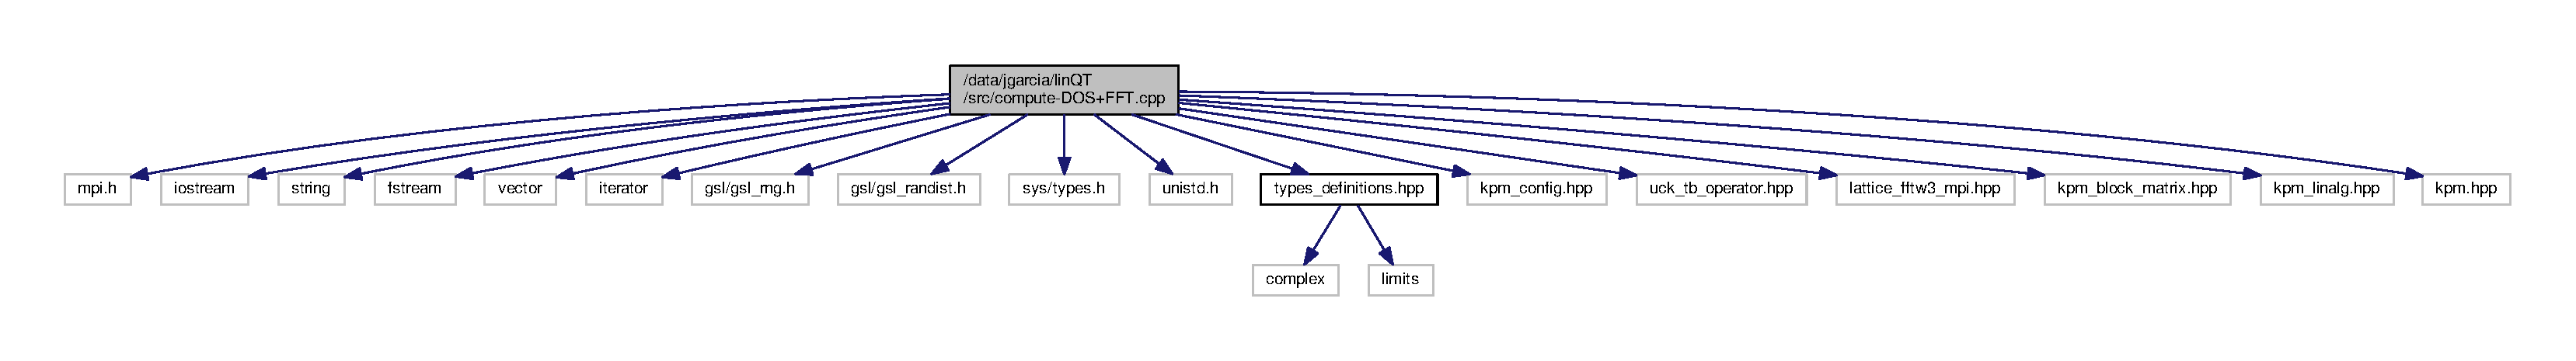
\includegraphics[width=350pt]{compute-DOS_09FFT_8cpp__incl}
\end{center}
\end{figure}
\subsection*{Functions}
\begin{DoxyCompactItemize}
\item 
int \hyperlink{compute-DOS_09FFT_8cpp_a0ddf1224851353fc92bfbff6f499fa97}{main} (int argc, char $\ast$argv\mbox{[}$\,$\mbox{]})\hypertarget{compute-DOS_09FFT_8cpp_a0ddf1224851353fc92bfbff6f499fa97}{}\label{compute-DOS_09FFT_8cpp_a0ddf1224851353fc92bfbff6f499fa97}

\begin{DoxyCompactList}\small\item\em The body of the function. \end{DoxyCompactList}\end{DoxyCompactItemize}


\subsection{Detailed Description}
This defines the compute-\/\+D\+O\+S+\+F\+FT function, which uses the kernel polynomial method and fast-\/fourier transform for computing the density of states in sparse systems. 

\begin{DoxyAuthor}{Author}
Jose H. Garcia (adamecius) 
\end{DoxyAuthor}
\begin{DoxyRefDesc}{Bug}
\item[\hyperlink{bug__bug000001}{Bug}]No know bugs. \end{DoxyRefDesc}

%--- End generated contents ---

% Index
\backmatter
\newpage
\phantomsection
\clearemptydoublepage
\addcontentsline{toc}{chapter}{Index}
\printindex

\end{document}
